\documentclass[a4paper,12pt]{article}
\usepackage{color}
\usepackage{graphicx}
\usepackage{subcaption}
\usepackage{amsmath}
 \graphicspath{ {./image/} }
\usepackage{natbib}
\begin{document}

\title{My first Document}
\author{Aisha Khatun}
\date{\today}
\maketitle

\pagenumbering{roman}
\tableofcontents
\listoftables
\listoffigures
\newpage
\pagenumbering{arabic}

\section{Introduction}
This is the introduction

\section{Tables}
{\begin{table}[ht]
\caption{Table of names and numbers}
\label{table1}
\begin{tabular}{|l|l|r|}
\hline
\textbf{Name} & \textbf{Number} \\
\hline
Aysha & 4110\\
\hline
Tanny & 2015331042\\
\hline
merged & 017565\\
\cline{1-1}
with this & \\
\hline
\end{tabular}
\caption{Country Table}
\label{table2}
%practical 3
\begin{tabular}{|c|c|c|c|}
\hline
\multicolumn{4}{|c|}{Country List}\\
\hline
Country Name & alpha 2 & alpha 3 & numeric code\\
\hline
Afghanistan & AF & AFG & 004\\
Albania & AL & ALB & 008\\
Algeria & DZ & DZA & 012\\
Angola & AO & AGO & 024 \\
\hline
\end{tabular}
\end{table}}

\section{Fonts}
My name is \textit{Aisha Khatun} , this is \textsl{slanted} and this is  in \textsc{smallcaps} also this is \underline{\textbf{both bold and underlined} }
\texttt{Aysha}  \textsf {Aysha }  \textrm{Aysha }
{\color{blue}coloring texts in various colors} {\color{cyan} that look good!}
{\huge all types}{\LARGE of sizes are }{\small are possible}\vspace{30pt}{\tiny are possible}{\scriptsize are possible}{\footnotesize are possible}{\normalsize are possible}
A list of works:
\begin{enumerate}
\item First thing
\item Second thing
\begin{itemize}
\item A sub-thing
\item Another sub-thing
\begin{itemize}
\item sub-sub thing
\item yet another
\begin{itemize}
\item[+] positive
\item[-] negative
\item[()] and words
\item[()] and more words
\end{itemize}
\end{itemize}
\end{itemize}
\item Third thing
\end{enumerate}

Believe that life is worth living% Note comic irony in the very first sentence
, and your belief will help create the fact
%Multiple consecutive spaces in LATEX are treated as a single space

new line  started here\\and another line break\newline also another newline

Trying out escape  characters like \# \$ \% \^ accent \^{} with this. how to enter the backslash? by typing \textbackslash textbackslash

Item \#A\textbackslash 642 costs \$8 \& is sold at a \~{}10\% profit

\section{Checkpoint Tables}
Assignment Table here.
{\begin{table}[ht]
\caption{Assignment table-1}
\center
\begin{tabular}{l|r|r}
Item & Quantity & Price (\$) \\
\hline
Nails & 500 & 0.34\\
Wooden boards & 100 & 4.00\\
Bricks & 240 & 11.50\\
\end{tabular}
\vspace{12pt}

\caption{Assignment table-2}
\begin{tabular}{l|ccc}
 & & Year &\\
\cline{2-4}
City & 2006 & 2007 & 2008\\
\hline
London & 1234 & 5687 & 9821\\
Berlin & 1234 & 5687 & 9821\\
Paris & 1234 & 5687 & 9821\\
\end{tabular}
\end{table}

\newpage

\section{Figures}
This part uses images\newline
\begin{figure}[h!]
\centering
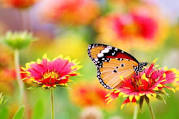
\includegraphics[width=1\textwidth]{myimage}
\caption{Here is my image}
\label{image-myimage}
\end{figure}

Figure \ref{image-myimage} shows my image.


\section{Multiple Figures}
\begin{figure}[h!]
\centering
\begin{subfigure}[b]{0.2\linewidth}
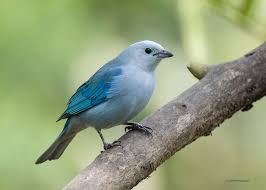
\includegraphics[width=\linewidth]{bird}
\caption{First Bird.}
\end{subfigure}
\begin{subfigure}[b]{0.2\linewidth}
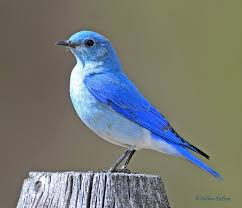
\includegraphics[width=\linewidth]{bird3}
\caption{Second  Bird.}
\end{subfigure}
\begin{subfigure}[b]{0.2\linewidth}
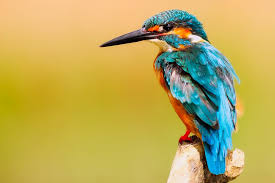
\includegraphics[width=\linewidth]{bird2}
\caption{Third  Bird.}
\end{subfigure}
\begin{subfigure}[b]{0.2\linewidth}
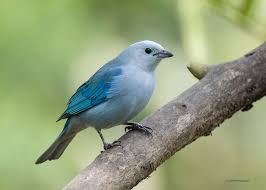
\includegraphics[width=\linewidth]{bird}
\caption{Repeated.}
\end{subfigure}
\caption{Some Birds together.}
\label{fig:Birds}
\end{figure}
Writing appear at the bottom

\newpage

\section{Bottom Figure}
This part uses images\newline
\begin{figure}[b!]
\centering
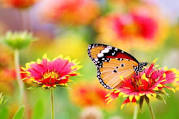
\includegraphics[width=1\textwidth]{myimage}
\caption{Here is my image}
\label{image-myimage1}
\end{figure}

Figure \ref{image-myimage1} shows my image.

\newpage

\section{New page Figure}
This part uses images\newline
\begin{figure}[p!]
\centering
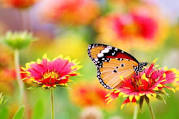
\includegraphics[width=1\textwidth]{myimage}
\caption{Here is my image}
\label{image-myimage2}
\end{figure}

Figure \ref{image-myimage2} shows my image.

\section{Practical 5}
\subsection{Equations}
$1+2=3$\\
Own line Equation
$$x+y=z$$

Numbered Equation
\begin{equation} %only one equation
ax+by=c
\end{equation}

\begin{eqnarray}
y=mx+c\\
ax+by=c\\
x1<=x<=x2 \hspace{15pt}y1<=y<=y2
\end{eqnarray}

\begin{eqnarray*}
y & = & mx+c\\
ax+by & = & c\\
x1< & = & x<=x2\\
 y1<=y< & = & y2
\end{eqnarray*}

\subsection{Symbols}
$$n^4$$
$$a_2$$
$$^nC_r$$
$$\frac{x}{y}$$
$$\frac{y}{\frac{3}{x}+b}$$
$$\sqrt{aysha^{100}}$$
$$\sqrt[100]{x^{100}+y^6}$$
$$\sum_{i=1}^n ({\frac{1}{2}})^i$$
$$\lim_{x \to \infty} f(x)$$
$$\int_a^b f(x)$$

\subsection{Matrices}
\begin{equation*}
\left[
\begin{matrix}
1 &  0 & 0 & a\\
0 & 1 & x & y\\
\end{matrix}
\right]
\end{equation*}

\subsection{Greek Letters}
$\alpha$\\
$\beta$\\
$\delta, \Delta$\\
%$\theta, \Theta$\\
$\mu$\\
$\pi, \Pi$\\
$\sigma, \Sigma$\\
$\phi, \Phi$\\
$\psi, \Psi$\\
$\omega, \Omega$\\

\subsection{CheckPoint 5}

\begin{equation}
e=mc^2
\end{equation}

\begin{equation}
\pi=\frac{c}{d}
\end{equation}

\begin{equation}
\frac{d}{dx}e^x=e^x
\end{equation}

\begin{equation}
\frac{d}{dx}\int_0^\infty f(s)ds=f(x)
\end{equation}

\begin{equation}
f(x)=\sum_t=0^\infty \frac{f^{(t)}(0)}{i!}x^t
\end{equation}

\begin{equation}
x=\sqrt{\frac{x_t}{z}y}
\end{equation}

\begin{equation}
\lim_{x \to \infty} exp(-x)=0
\end{equation}

\begin{equation}
\left[
\begin{matrix}
1 & 2 & 3 & 4 & 5\\
3 & 4 & 5 & 6 &  7\\
5 & 6 & 7 & 8 & 9\\
\end{matrix}
\right]
\end{equation}

\section{Bibliography}

Citation is \citep{Birdetal2001}\\
Citation is \cite{goldberg1988genetic}\\
Reference is not showing\nocite{goldberg1988genetic}\\
With Page Number \cite[p. 215]{Birdetal2001}\\
Multiple Citation \cite{goldberg1988genetic,nasrabadi2007pattern,rasmussen2004gaussian,Birdetal2001}\\

\section{Methods}

\subsection{Stage 1}
\label{sec1}
The first part of the methods.

\subsection{Stage 2}
The second part of the methods.

\section{Results}
Here are my results. Referring to section \ref{sec1} on page \pageref{sec1} and the first table practice \ref{table1} on page \pageref{table1} 


\bibliographystyle{plainnat}
\bibliography{lab_1}
\end{document}